\documentclass[]{../template/Report}%方括号内写yuxi即生成预习报告\documentclass[yuxi]{../template/Report}
\settemplatedir{../template/}%设置模板路径

\exname{等厚干涉} %实验名称
\extable{} %实验桌号
\instructor{张俊香} %指导教师
\class{} %班级
\name{} %姓名
\stuid{} %学号

\nyear{} %年
\nmonth{} %月
\nday{} %日
\nweekday{} %星期几，e.g. \nweekday{三}
\daypart{}%上午/下午

\redate{} %如有实验补做，补做日期
\resitu{} %情况说明：

\begin{document}
\maketitle%输出封面

\section{预习报告（10分）}
（注：将已经写好的“物理实验预习报告”内容拷贝过来）

\subsection{实验综述（5分）}
（自述实验现象、实验原理和实验方法，包括必要的光路图、电路图、公式等。不超过500字。）
\subsubsection{实验原理}
\textbf{(1)光的相干条件：}频率相同；振动方向相同；相位差恒定；光程差远小于相干长度
\par

\textbf{(2)获取相干光的两种途径：}
\par
分波面法：点光源的波阵面分割为两部分，这两部分分别通过两个光具组，经反射、折射或衍射后交迭起来，在一定区域形成干涉。
\par
分振幅法:当一束光投射到两种透明媒质的分界面上，光一部分反射，另一部分折射，若将它们再次汇聚后就会形成干涉。
\par

\textbf{(3)牛顿环光程差公式}
\[
\Delta = 2ne + \frac{\lambda}{2}
\]
\par
n：薄膜折射率（空气膜：n = 1）  e：薄膜厚度 $\frac{\lambda}{2}$：半波损失（光从光疏媒质射向光密媒质时反射产生）
\par

\textbf{(4)牛顿环明暗条纹条件/特点}
\par
明条纹：$\Delta = k\lambda$
\par
暗条纹：$\Delta = (2k+1)\frac{\lambda}{2}$
\par
牛顿环条纹特点：等厚干涉条纹是薄膜厚度相等处的点构成的同一条纹。在牛顿环实验中，空气膜厚度e与透镜曲率半径R、条纹半径r满足关系$r^2 = 2Re$，条纹为以接触点为中心的同心圆。
\par

\textbf{(5)实验一测量公式}
\begin{figure}[H]
    \centering
    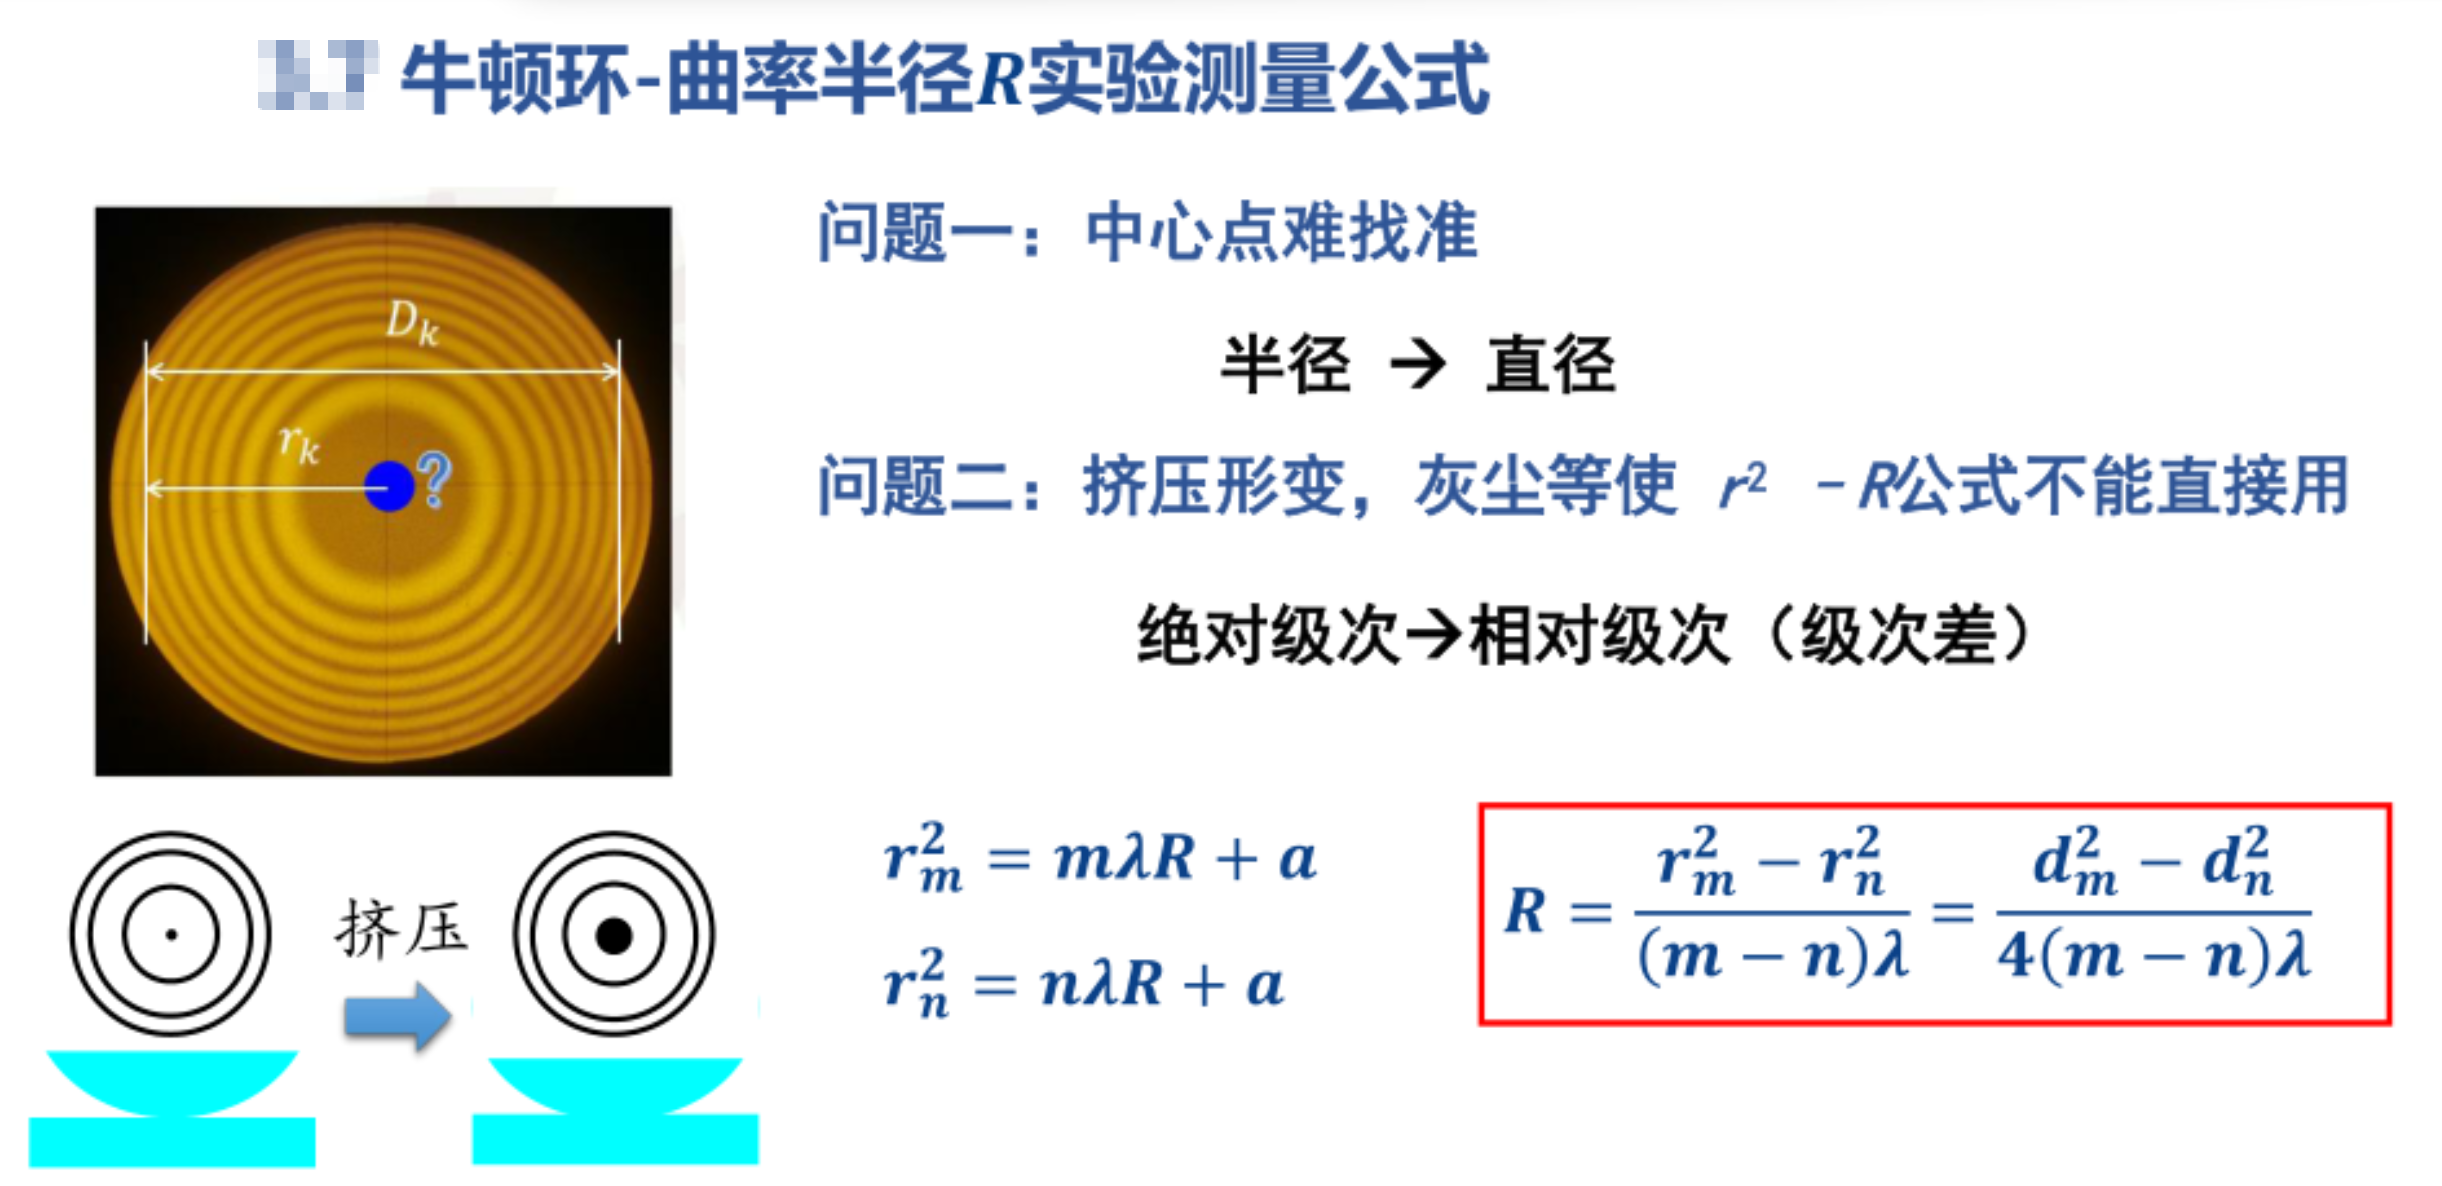
\includegraphics[width=0.6\textwidth]{figures/实验原理_测量公式.png}
    \caption{实验一原理}
\end{figure}

\textbf{(6)测量薄膜厚度（实验二）原理}
\begin{figure}[H]
    \centering
    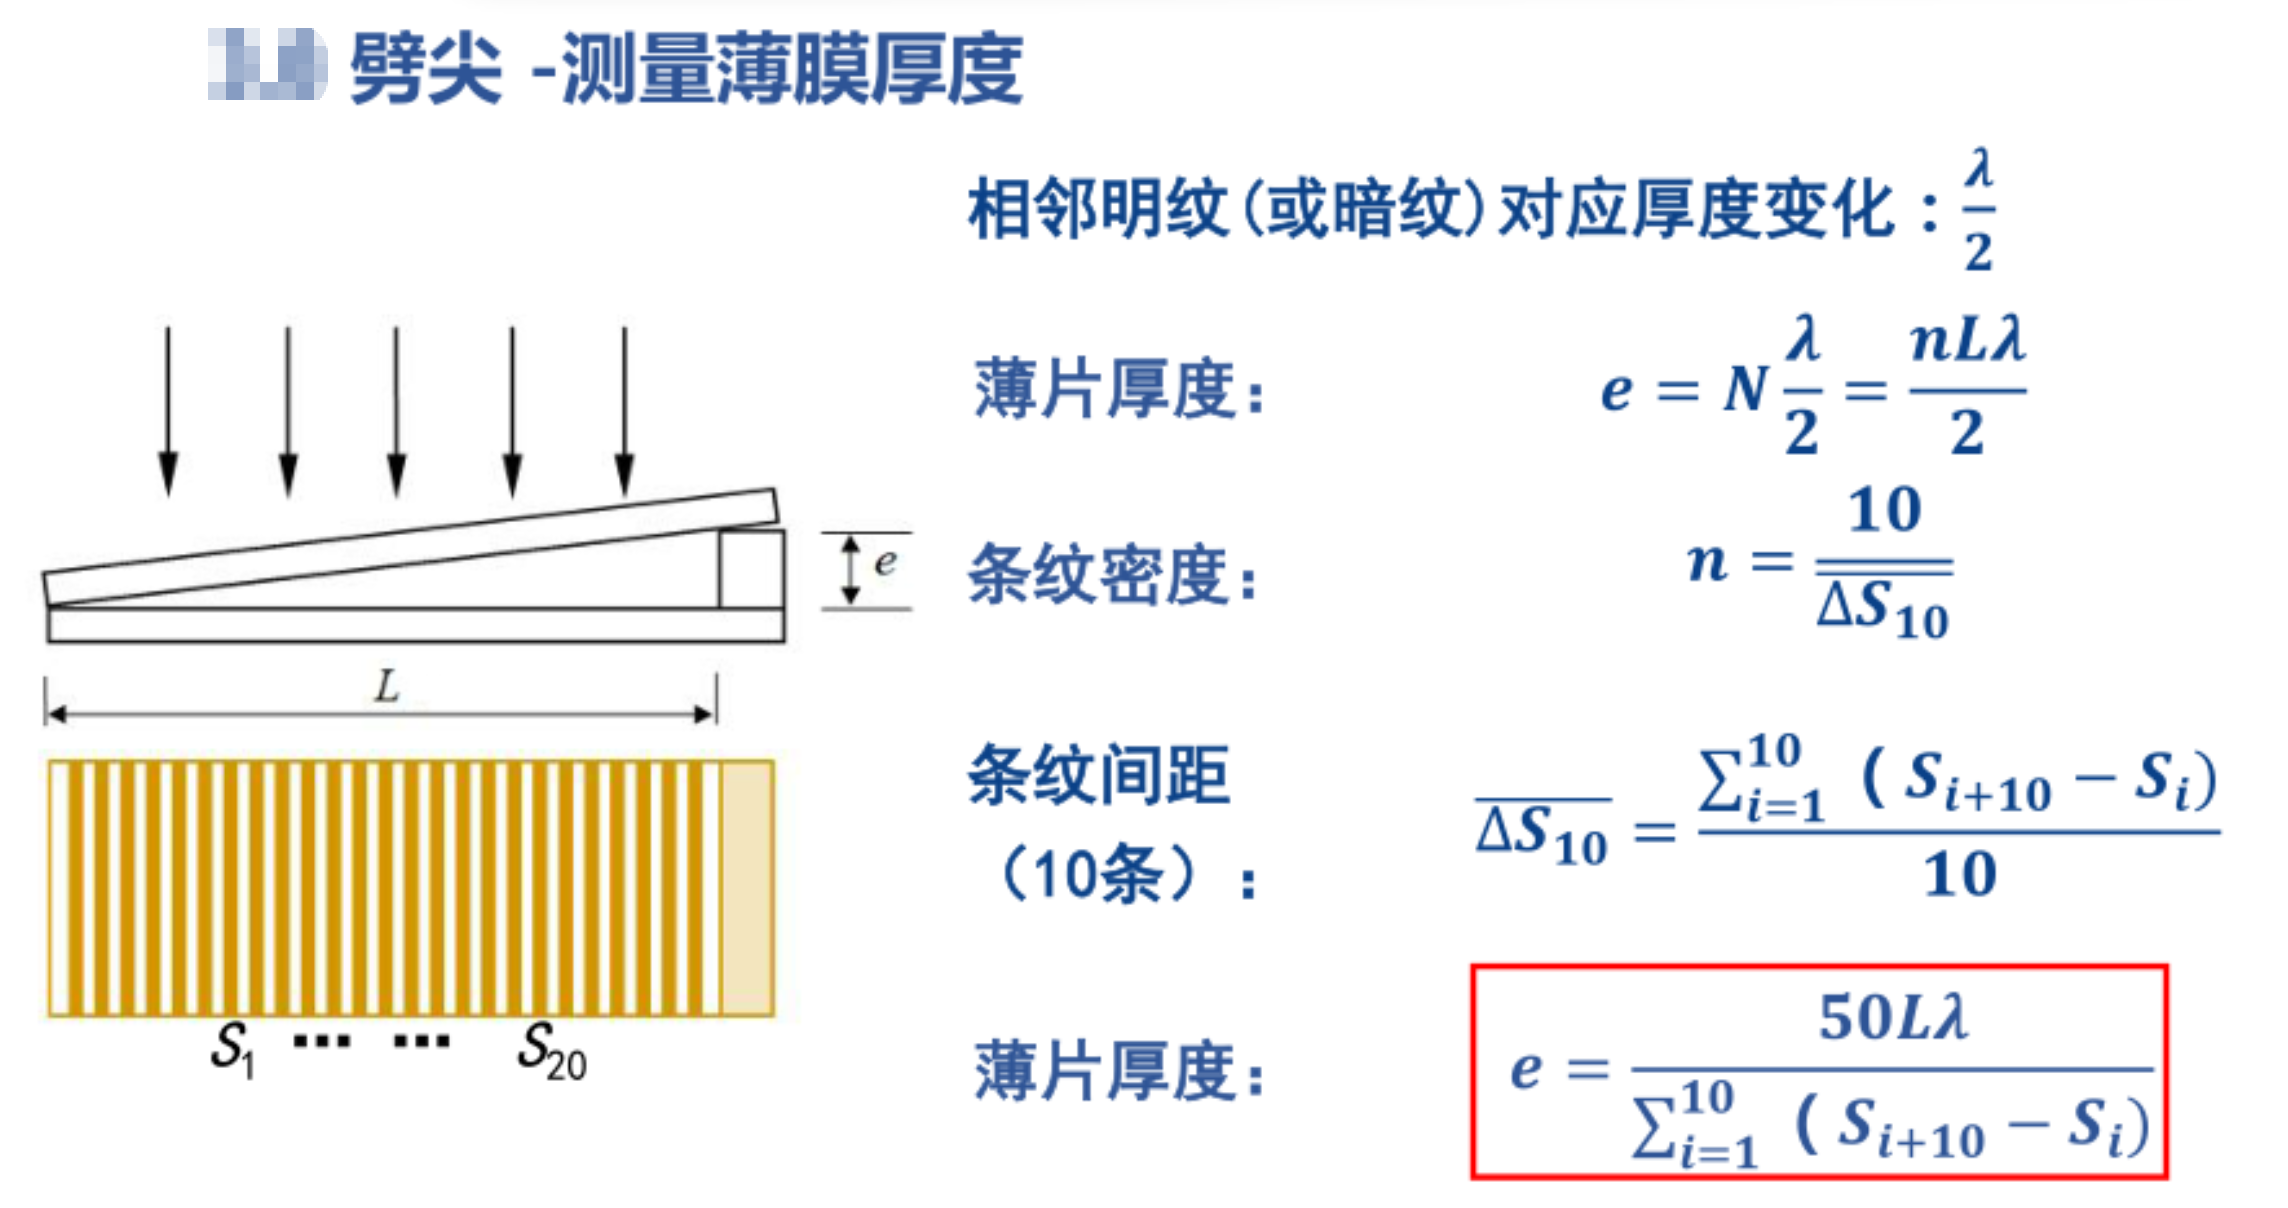
\includegraphics[width=0.6\textwidth]{figures/实验二原理.png}
    \caption{实验二原理}
\end{figure}



\subsubsection{实验步骤}
\textbf{(1)实验一：牛顿环曲率半径}
\par
1、打开钠灯，调节半反半透玻片，使显微镜视场较亮
\par
2、调节目镜看清目镜筒中的叉丝(消除视差)
\par
3、微调牛顿环装置
\par
4、转动测微鼓轮，使十字叉丝交点接近牛顿环中心
\par
5、旋转鼓轮，记录16个暗环两侧位置(粗细合适，能分辨，空程差)
\par
6、计算透镜曲率半径
\par

\textbf{(2)实验二：测量薄膜厚度}
\par
1、测量劈尖到待测薄膜边缘的距离L
\par
2、测量条纹数据，记录标尺读数
\par
3、计算e

\subsection{实验重点（3分）}
（简述本实验的学习重点，不超过100字。）
\subsubsection{理解牛顿环和劈尖干涉条纹的成因}
\subsubsection{学习用等厚干涉法测量平凸透镜的曲率半径和薄膜厚度}
\subsubsection{学会使用读数显微镜}


\subsection{实验难点（2分）}
（简述本实验的实现难点，不超过100字。）
\subsubsection{条纹清晰度与稳定性控制}
\textbf{(1)调焦与对准困难：}需确保入射光垂直投射到薄膜表面（如牛顿环实验中平凸透镜与平玻璃的接触点需居中），否则条纹会出现畸变或模糊。若光路倾斜，干涉条纹对比度下降，甚至无法形成同心圆或平行直条纹。
\par
\textbf{(2)振动干扰：}实验装置对微小振动敏感，环境振动（如桌面晃动、气流）会导致条纹漂移，难以稳定读数。

\subsubsection{附加光程差的消除}
薄膜表面不洁净（如牛顿环实验中玻璃表面有灰尘）会引入额外厚度差，导致光程差计算偏差；反射面存在微小倾角时，等厚条纹会偏离理论位置，需反复调整装置保证“等厚”条件。

\subsubsection{读数与数据采集具有一定的难度}
靠近中心的条纹较粗且稀疏，边缘条纹密集且细，读数显微镜十字叉丝对准条纹边缘时易产生主观偏差。

\begin{fullreportonly}
\section{原始数据（20分）}
（将有老师签名的“自备数据记录草稿纸”的扫描或手机拍摄图粘贴在下方，完整保留姓名，学号，教师签字和日期。）
% \begin{figure}[H]
%     \centering
%     
\includegraphics[width=0.6\textwidth]{figures/原始数据.jpg}
%     \caption{实验原始数据}
% \end{figure}

\section{结果与分析（60分）}
\subsection{数据处理与结果（30分）}
（列出数据表格、选择适合的数据处理方法、写出测量或计算结果。）
\subsubsection{实验一：牛顿环实验测量与数据处理}
计算公式：
\[
R = \frac{d_m^2-d_n^2}{4(m-n)\lambda} \quad\quad  \lambda = 589.3nm
\]
\par
\begin{table}[H]
    \centering
    \caption{实验一：牛顿环实验数据记录与处理}
    \begin{tabular}{|c|c|c|c|c|c|c|}
        \hline
        \textbf{圈数号(k)} & \textbf{$d_\text{右}(mm)$} & \textbf{$d_\text{左}(mm)$} & \textbf{$d_\text{右}-d_\text{左} (mm)$} & \textbf{直径平方$d_k^2(mm^2)$} & \textbf{相隔6圈直径平方数之差} & \textbf{R(m)}  \\
        \hline
        12 & 26.302 & 31.572 & 5.270 & 27.773 & $d_{12}^2-d_6^2=14.799$ & 1.046  \\
        \hline
        11 & 26.579 & 31.615 & 5.036 & 25.361 & $d_{11}^2-d_5^2=14.603$ & 1.033  \\
        \hline
        10 & 26.788 & 31.570 & 4.782 & 22.868 & $d_{10}^2-d_4^2=14.660$ & 1.037  \\
        \hline
        9 & 26.990 & 31.526 & 4.536 & 20.575 & $d_9^2-d_3^2=14.872$ & 1.052  \\
        \hline
        8 & 27.118 & 31.400 & 4.282 & 18.336 & $d_8^2-d_2^2=14.320$ & 1.013  \\
        \hline
        7 & 27.240 & 31.184 & 3.944 & 15.555 & $d_7^2-d_1^2=14.677$ & 1.038  \\
        \hline
        6 & 27.400 & 31.002 & 3.602 & 12.974 & &  \\
        \hline
        5 & 27.534 & 30.814 & 3.280 & 10.758 & \textbf{平均值$\bar{R}$} & 1.037 \\
        \hline
        4 & 27.659 & 30.524 & 2.865 & 8.208 & \textbf{A类不确定度$\mu_R$} & 0.005 \\
        \hline
        3 & 27.814 & 30.202 & 2.388 & 5.703 & &  \\
        \hline
        2 & 27.919 & 29.923 & 2.004 & 4.016 & &  \\
        \hline
        1 & 28.026 & 28.963 & 0.937 & 0.878 & &  \\
        \hline
    \end{tabular}
\end{table}
故$R = 1.037 \pm 0.005$(m)

\subsubsection{实验二：劈尖实验测量与数据处理}
计算公式：
\[
e = nL\frac{\lambda}{2} \quad n = \frac{1}{\Delta s} = \frac{10}{s_{x+10}-s_x} \quad L = 43.2mm \quad \lambda = 589.3nm
\]
\[
e = \frac{5L \lambda}{s_{x+10}-s_x}
\]
\[
e = \frac{50L \lambda}{\sum_{x=1}^{10}(s_{x+10}-s_x)}
\]
\begin{table}[H]
    \centering
    \caption{实验二：劈尖实验数据记录与处理}
    \begin{tabular}{|c|c|c|c|}
        \hline
        \textbf{标尺读数S(mm)} & \textbf{标尺读数S(mm)} & \textbf{$S_{x+10}-S_x$(mm)} & \textbf{e(mm)}  \\
        \hline
        $s_1 = 20.410$ & $s_{11} = 22.736$ & $s_{11}-s_1 = 2.326$ & $5.472 \times 10^{-2}$  \\
        \hline
        $s_2 = 20.645$ & $s_{12} = 23.001$ & $s_{12}-s_2 = 2.356$ & $5.403 \times 10^{-2}$  \\
        \hline
        $s_3 = 20.858$ & $s_{13} = 23.229$ & $s_{13}-s_3 = 2.371$ & $5.369 \times 10^{-2}$ \\
        \hline
        $s_4 = 21.104$ & $s_{14} = 23.491$ & $s_{14}-s_4 = 2.387$ & $5.333 \times 10^{-2}$  \\
        \hline
        $s_5 = 21.310$ & $s_{15} = 23.730$ & $s_{15}-s_5 = 2.420$ & $5.260 \times 10^{-2}$  \\
        \hline
        $s_6 = 21.568$ & $s_{16} = 23.980$ & $s_{16}-s_6 = 2.412$ & $5.277 \times 10^{-2}$  \\
        \hline
        $s_7 = 21.797$ & $s_{17} = 24.220$ & $s_{17}-s_7 = 2.423$ & $5.253 \times 10^{-2}$  \\
        \hline
        $s_8 = 22.045$ & $s_{18} = 24.478$ & $s_{18}-s_8 = 2.433$ & $5.232 \times 10^{-2}$  \\
        \hline
        $s_9 = 22.284$ & $s_{19} = 24.740$ & $s_{19}-s_9 = 2.456$ & $5.183 \times 10^{-2}$  \\
        \hline
        $s_{10} = 22.521$ & $s_{20} = 25.010$ & $s_{20}-s_{10} = 2.489$ & $5.114 \times 10^{-2}$  \\
        \hline
        \textbf{平均值$\bar{e}$(mm)} & 5.290 $\times 10^{-2}$ & \textbf{A类不确定度$\mu_e$} & 0.107 \\
        \hline
    \end{tabular}
\end{table}
故$e = (5.290 \pm 0.107) \times 10^{-2}$(mm)

\subsection{误差分析（20分）}
（运用测量误差、相对误差或不确定度等分析实验结果，写出完整的结果表达式，并分析误差原因。）
\subsubsection{仪器误差}
\textbf{(1)读数显微镜精度限制：}显微镜最小分度值通常为0.01mm，估读时易产生±0.001mm的偶然误差。
\par
\textbf{(2)光学元件缺陷：}牛顿环装置中平凸透镜曲率半径不均匀、平面玻璃不平整，或劈尖装置两玻璃板不平行。
\par
\textbf{(3)装置稳定性不足：}牛顿环装置金属框架松动，导致平凸透镜与平面玻璃接触点偏移。

\subsubsection{测量误差}
\textbf{(1)条纹对准误差：}读取条纹直径（如牛顿环暗纹）时，叉丝未准确对准条纹中心，或条纹本身模糊、变形。
\par
\textbf{(2)条纹级次误判：}牛顿环中心暗斑可能因灰尘存在而变为亮斑，导致级次k计数错误。
\par
\textbf{(3)回程差未消除：}移动显微镜时，未沿同一方向连续测量（如先向左再向右移动），导致丝杆间隙误差。

\subsubsection{环境因素误差}
\textbf{(1)温度变化影响：}温度变化导致空气折射率 n 改变。
\par
\textbf{(2)振动干扰：}实验台震动导致条纹漂移，无法稳定读数。
\par
\textbf{(3)空气对流影响：}空气流动引起局部折射率不均匀，导致条纹变形或抖动。


\subsection{实验探讨（10分）}
（对实验内容、现象和过程的小结，不超过100字。）
\par
通过本次实验，我加深理解了牛顿环和劈尖干涉条纹的成因，学会了用等厚干涉法测量平凸透镜的曲率半径和薄膜厚度，掌握了读数显微镜的使用。
\par
实验刚开始时，我未能快速找到劈尖的干涉条纹。后来经过耐心地反复调试——旋转透镜和移动载玻片，最后成功在视野里看到清晰的干涉条纹。这一过程十分考验我的耐心，这对我来说也是一次实践锻炼。

\section{思考题（10分）}
（解答教材或讲义或老师布置的思考题，请先写题干，再作答。）
\subsection{如何消除读数显微镜引起的空程差？}
\textbf{(1)测量过程中鼓轮单向转动}
\par
读数显微镜的鼓轮与丝杆之间存在机械间隙，若中途反向转动，会导致刻度变化与实际移动不同步。因此，测量全程需保持鼓轮沿同一方向转动（如仅顺时针或逆时针），避免中途换向。
\par

\textbf{(2)正式读数前预转鼓轮}
\par
为确保丝杆与螺母紧密贴合，正式读数前需将鼓轮预先转动几圈，待显微镜镜筒稳定移动后再开始记录数据，以消除初始间隙导致的空程误差。

\subsection{为什么随着牛顿圈半径增大，条纹越来越密？}
牛顿环由平凸透镜下表面与平面玻璃上表面之间的空气薄膜产生等厚干涉形成。设平凸透镜曲率半径为R，第k级暗纹半径为$r_k$，空气膜厚度为h。根据几何关系，当 h<<R 时，有：
\[
r_k \approx 2Rh_k  =>  h_k = \frac{r_k^2}{2R}
\]
\par
暗纹满足光程差条件：
\[
2h_k + \frac{\lambda}{2} = (2k+1)\frac{\lambda}{2} \quad (k = 0,1,2,...)
\]
\par
将两式化简得：
\[
r_k = \sqrt{kR\lambda}
\]
\par
由上式可得：条纹半径$r_k$与级次k的平方根成正比。随着k增大（即半径$r_k$增大），$\Delta r$逐渐减小。
\par
所以牛顿环条纹从中心向外，相邻条纹的间距越来越小，表现为条纹逐渐变密。

\subsection{在透射光中是否也可以观测干涉条纹？}
可以观测到干涉条纹。
\par
等厚干涉的核心是薄膜上下表面反射（或透射）的两束光因光程差满足干涉条件而形成条纹。对于牛顿环等典型等厚干涉装置，当光垂直入射时，透射光与反射光类似，同样会在薄膜（如空气膜）的不同厚度处形成干涉条纹。
\par
从光程差角度分析：透射光的两束相干光分别来自薄膜上表面的直接透射光和下表面反射后再透射的光。与反射光相比，透射光的半波损失情况不同（反射光中通常存在额外半波损失，而透射光中一般无半波损失），因此透射光的干涉条纹与反射光条纹互补——即反射光中的明纹对应透射光中的暗纹，反之亦然。
\par
不过，由于透射光的光强通常较弱（大部分光能量被反射），条纹对比度较低，实验中更常用反射光观测以获得清晰条纹。但理论上，通过适当增强入射光强度或使用高灵敏度探测器，透射光干涉条纹是可以被观测到的。

\end{fullreportonly}
\insertnotes
\end{document}